\documentclass[preview]{standalone}

\usepackage{amsmath}
\usepackage{amssymb}
\usepackage{tikz}
\usepackage{float}
\usepackage{xcolor}
\usepackage{stellar}
\usepackage{definitions}

\begin{document}

\id{differentiation-basic-results}
\genpage

\section{L'Hôpital Rule}

\begin{snippettheorem}{hopital-rule}{L'Hôpital Rule}
    Let \(f(x)\) and \(g(x)\) be differentiable in an open interval \(I\) except
    possibly at \(x=c\), if
    \[
        \lim_{x\to c} f(x) = \lim_{x\to c} g(x) = 0 \text { or } \pm \infty, \quad g(x\in I) \neq 0
    \]
    then
    \[
        \lim_{x\to c} \frac{f(x)}{g(x)} = \lim_{x\to c} \frac{f'(x)}{g'(x)} 
    \]
    if such limit exists.
\end{snippettheorem}

\section{Intermediate value Theorem}

\begin{snippettheorem}{intermediate-value-theorem}{Intermediate value Theorem}
    A \function \(f\) continuous on an interval \([a;b]\) will take
    every value in the interval \([f(a);f(b)]\).
\end{snippettheorem}

\section{Bolzano's Theorem}

\begin{snippettheorem}{bolzano-theorem}{Bolzano's Theorem}
    If \(f(x)\) is continuous on \([a;b]\) and \(f(a)\cdot f(b) <0\) then there is a root.
    \[
        f(a)\cdot f(b) <0 \implies \exists c \in [a;b] \mid f(c) = 0
    \]
\end{snippettheorem}

\section{Weierstrass Theorem}

\begin{snippettheorem}{weierstrass-theorem}{Weierstrass Theorem}
    If \(f(x)\) is continuous in \([a;b]\) then the function will have a maxima and a minima.
\end{snippettheorem}

\section{Rolle's Theorem}

\begin{snippettheorem}{rolle-theorem}{Rolle's Theorem}
    Suppose that \(f(x)\) is continuous on \([a;b]\) and differentiable on \((a;b)\).
    \[
        f(a)=f(b) \implies \exists \,c \suchthat f'(c) = 0, \quad
        a < c < b
    \]
\end{snippettheorem}

\section{Mean Value Theorem}

\begin{snippettheorem}{mean-value-theorem}{Mean Value Theorem}
    Suppose \(f(x)\) is a \function continuous on \([a;b]\) and
    differentiable on \((a;b)\), there there exists a number \(c\) such that
    \[
        f'(x)=\frac{f(b)-f(a)}{b-a}, \quad a<c<b
    \]
\end{snippettheorem}

\begin{snippet}{mean-value-theorem-illustration}
    \begin{minipage}{0.5\textwidth}
        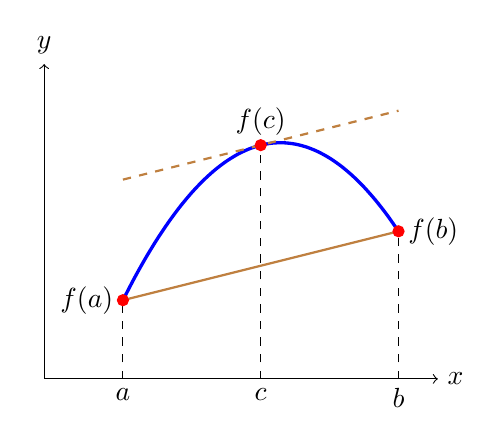
\begin{tikzpicture}[
            declare function={
                func(\x) = - \x * \x * 0.5 + 3 * \x - 1.5;
                a = 1;
                b = 4.5;
                c = 2.75;
                Width=5;
                Height=4;
                m = {(func(b) - func(a)) / (b-a)};
            }
        ]

            \draw[domain=a:b, smooth, variable=\x, blue, very thick] plot ({\x}, {func(\x)});
            \draw[domain=a:b, smooth, variable=\x, brown, thick, dashed] plot ({\x}, {m * \x + 2.28125});
            
            \draw[-, dashed] (a, 0) node[below] {\(a\)} -- (a, {func(a)}) node[left] {\(f(a)\)};
            \draw[-, dashed] (b, 0) node[below] {\(b\)} -- (b, {func(b)}) node[right] {\(f(b)\)};
            \draw[-, dashed] (c, 0) node[below] {\(c\)} -- (c, {func(c)});

            \draw[-, brown, thick] (a, {func(a)}) -- (b, {func(b)});
            
            \filldraw [red] (a,{func(a)}) circle (2pt);
            \filldraw [red] (b,{func(b)}) circle (2pt);
            \filldraw [red] (c,{func(c)}) circle (2pt) node[above, black] {\(f(c)\)};

            \draw[->] (0, 0) -- (Width, 0) node[right] {\(x\)};
            \draw[->] (0, 0) -- (0, Height) node[above] {\(y\)};
        \end{tikzpicture}
    \end{minipage}
    \begin{minipage}{0.5\textwidth}
        The mean value on the interval can be represented by the {\color{brown} secant} line.
        What this means is that the interval contains a point whose tangent is equal to the secant.
        \\\\
        Note that if \(f(a) = f(b)\) this is Rolle's theorem.
    \end{minipage}
\end{snippet}

\end{document}